\documentclass[12pt]{article}

%% preamble: Keep it clean; only include those you need
\usepackage{amsmath}
\usepackage[margin = 1in]{geometry}
\usepackage{graphicx}
\usepackage{booktabs}
\usepackage{natbib}

% for space filling
\usepackage{lipsum}
% highlighting hyper links
\usepackage[colorlinks=true, citecolor=blue]{hyperref}


%% meta data

\title{Electronic Sports: Winner Prediction}
\author{Hao Ding\\
  Department of Statistics\\
  University of Connecticut
}

\begin{document}
\maketitle

\begin{abstract}
	
This paper explores factors influencing player success in the popular online multiplayer battle royale game, PlayerUnknown's Battlegrounds (PUBG). Utilizing data from the PUBG Developer API, which includes information from over 65,000 recorded games, we employ correlation analysis, feature importance from tree-based models, and recursive feature elimination to identify key elements impacting player performance. The dataset encompasses various metrics such as assists, boosts, revives, damage dealt, team kills, kill place, distance traveled, weapons acquired, match duration, and win place percentile. Our analysis reveals correlations between different factors and highlights the significance of kills and walk distance in achieving better win placements. The methods section details the approach, including the use of ensemble models like Random Forest and Gradient Boosting, as well as deep learning models for predictive tasks. The discussion emphasizes the need for a large and diverse dataset, periodic model updates due to game dynamics, collaboration with PUBG experts, and the inherent unpredictability of player strategies. While machine learning models offer valuable insights, they should be interpreted cautiously, recognizing the game's dynamic nature and unpredictable elements.  

\end{abstract}


\section{Introduction}
\label{sec:intro}

PUBG (PlayerUnknown's Battlegrounds). PUBG is a popular online multiplayer battle royale game developed and published by PUBG Corporation, a subsidiary of South Korean video game company Bluehole. It was inspired by the Japanese film "Battle Royale" and released in March 2017.

In PUBG, up to 100 players parachute onto an island and scavenge for weapons and equipment to eliminate others while avoiding getting eliminated themselves. The game features a shrinking play area that forces players into closer proximity, creating intense encounters. The last player or team standing wins the match.

PUBG gained immense popularity shortly after its release, contributing to the rise of the battle royale genre in gaming. The game is available on various platforms, including PC, Xbox, PlayStation, and mobile devices. PUBG Corporation has also organized esports events, such as the PUBG Global Championship, where professional players and teams compete for significant prizes


Our goal is to analyze this dataset to figure out which specific factors or behaviors lead to more kills or longer game life, which leads to player wins.



% roadmap
The rest of the paper is organized as follows.
The data will be presented in Section~\ref{sec:data}.
The methods are described in Section~\ref{sec:meth}.
The results are reported in Section~\ref{sec:resu}.
A discussion concludes in Section~\ref{sec:disc}.


\section{Data}
\label{sec:data}

Data from the PUBG Developer API, it  is a official game data. There are over 65,000 games recorded in this database.  

Assists - 			Number of enemy players this player damaged that were killed by teammates.
Boosts -          		Number of boost items used.
Revives - 	     		Number of times this player revived teammates.
Heals - 	     		Number of healing items used.
Damage Dealt - 		Total damage dealt. Note: Self inflicted damage is subtracted.
TeamKills - 		Number of times this player killed a teammate.
Kill Place - 		Ranking in match of number of enemy players killed.
kills - 			Number of enemy players killed.
Ride Distance - 		Total distance traveled in vehicles measured in meters.
Swim Distance - 	Total distance traveled by swimming measured in meters.
Walk Distance - 	Total distance traveled on foot measured in meters.
Weapons Acquired - 	Number of weapons picked up.
Match Duration - 	Duration of match in seconds.
Win Place Perc -  	This is a percentile winning placement, where 1 corresponds to 1st place, and 0 corresponds to last place in the match.




\section{Methods}
\label{sec:meth}

Like we  said before,  correlation analysis, Feature importance from tree-based modes and recursive feature elimination are main method to select data to reduce the dataset size. Then, we split the data with training and testing sets. Choose appropriate machine learning models. Given that this is a predictive task with multiple features, ensemble methods like Random Forest or Gradient Boosting might be effective. Additionally, deep learning models like neural networks could be explored. we should train the chosen model using the training set.

\begin{figure}[t]
	\centering
	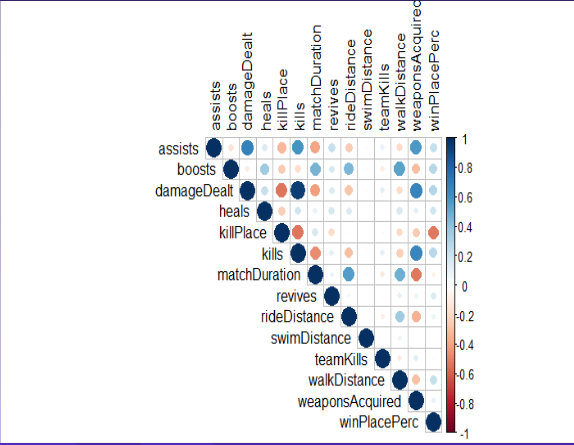
\includegraphics[width=\textwidth]{Correlation.png}
	\caption{The Correlation between each Factor}
	\label{fig:Correlation}
\end{figure}

Figure~\ref{fig:Correlation} shows Correlation between each factors so that we can select the important factor. 

\begin{figure}[t]
	\centering
	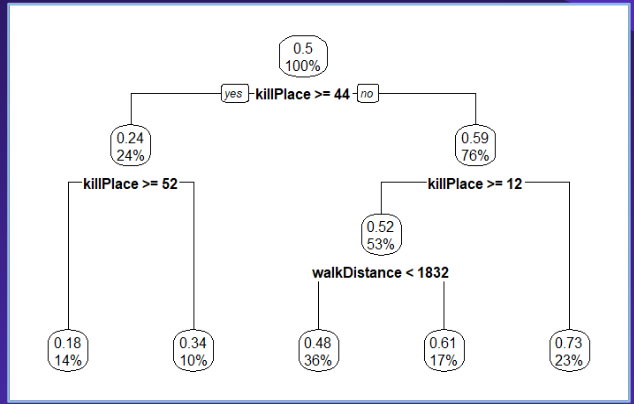
\includegraphics[width=\textwidth]{tree.png}
	\caption{The Tree Method }
	\label{fig:tree}
\end{figure}


Figure~\ref{fig:tree} shows Higher kills and more WalkDistance will  lead to better win placement. 







\section{Discussion}
\label{sec:disc}

We can choose several models, and compared with the accuracy of those models, and we will choose the highest accuracy model as our final model to predict whether the players or teams can win. So, we need to consider more detail for different modeling methods that will be lots of work.
Second point is ensure that we have a sufficiently large and diverse dataset training a robust model.
Since this is a video game, PUBG is a dynamic game with constant updates and changes. The model might need periodic updates to adapt to the evolving game environment.

If it is possible, we should work closely with PUBG experts to gain insights into the specific dynamics of the game that may not be immediately evident from the data.

Also we should emphasize a important factor, while machine learning models can provide valuable insights, predicting the outcome of a PUBG  involves various unpredictable factors, including player strategies, teamwork, and unexpected events during matches. Always interpret the model's predictions cautiously and use them as a supplementary tool rather than a definitive source for predicting winners.




\bibliography{refs}
\bibliographystyle{mcap}

\end{document}